\chapter{ بخش اول}
در این قسمت به کمک جعبه‌ابزار SISO یک کنترل کننده از خانواده PID برای سیستم در طراحی شد. خروجی پله واحد سیستم مدار بسته در حضور کنترل‌کننده PID در شکل
\ref{PID}
آورده شده است.
 \begin{figure}[H]
	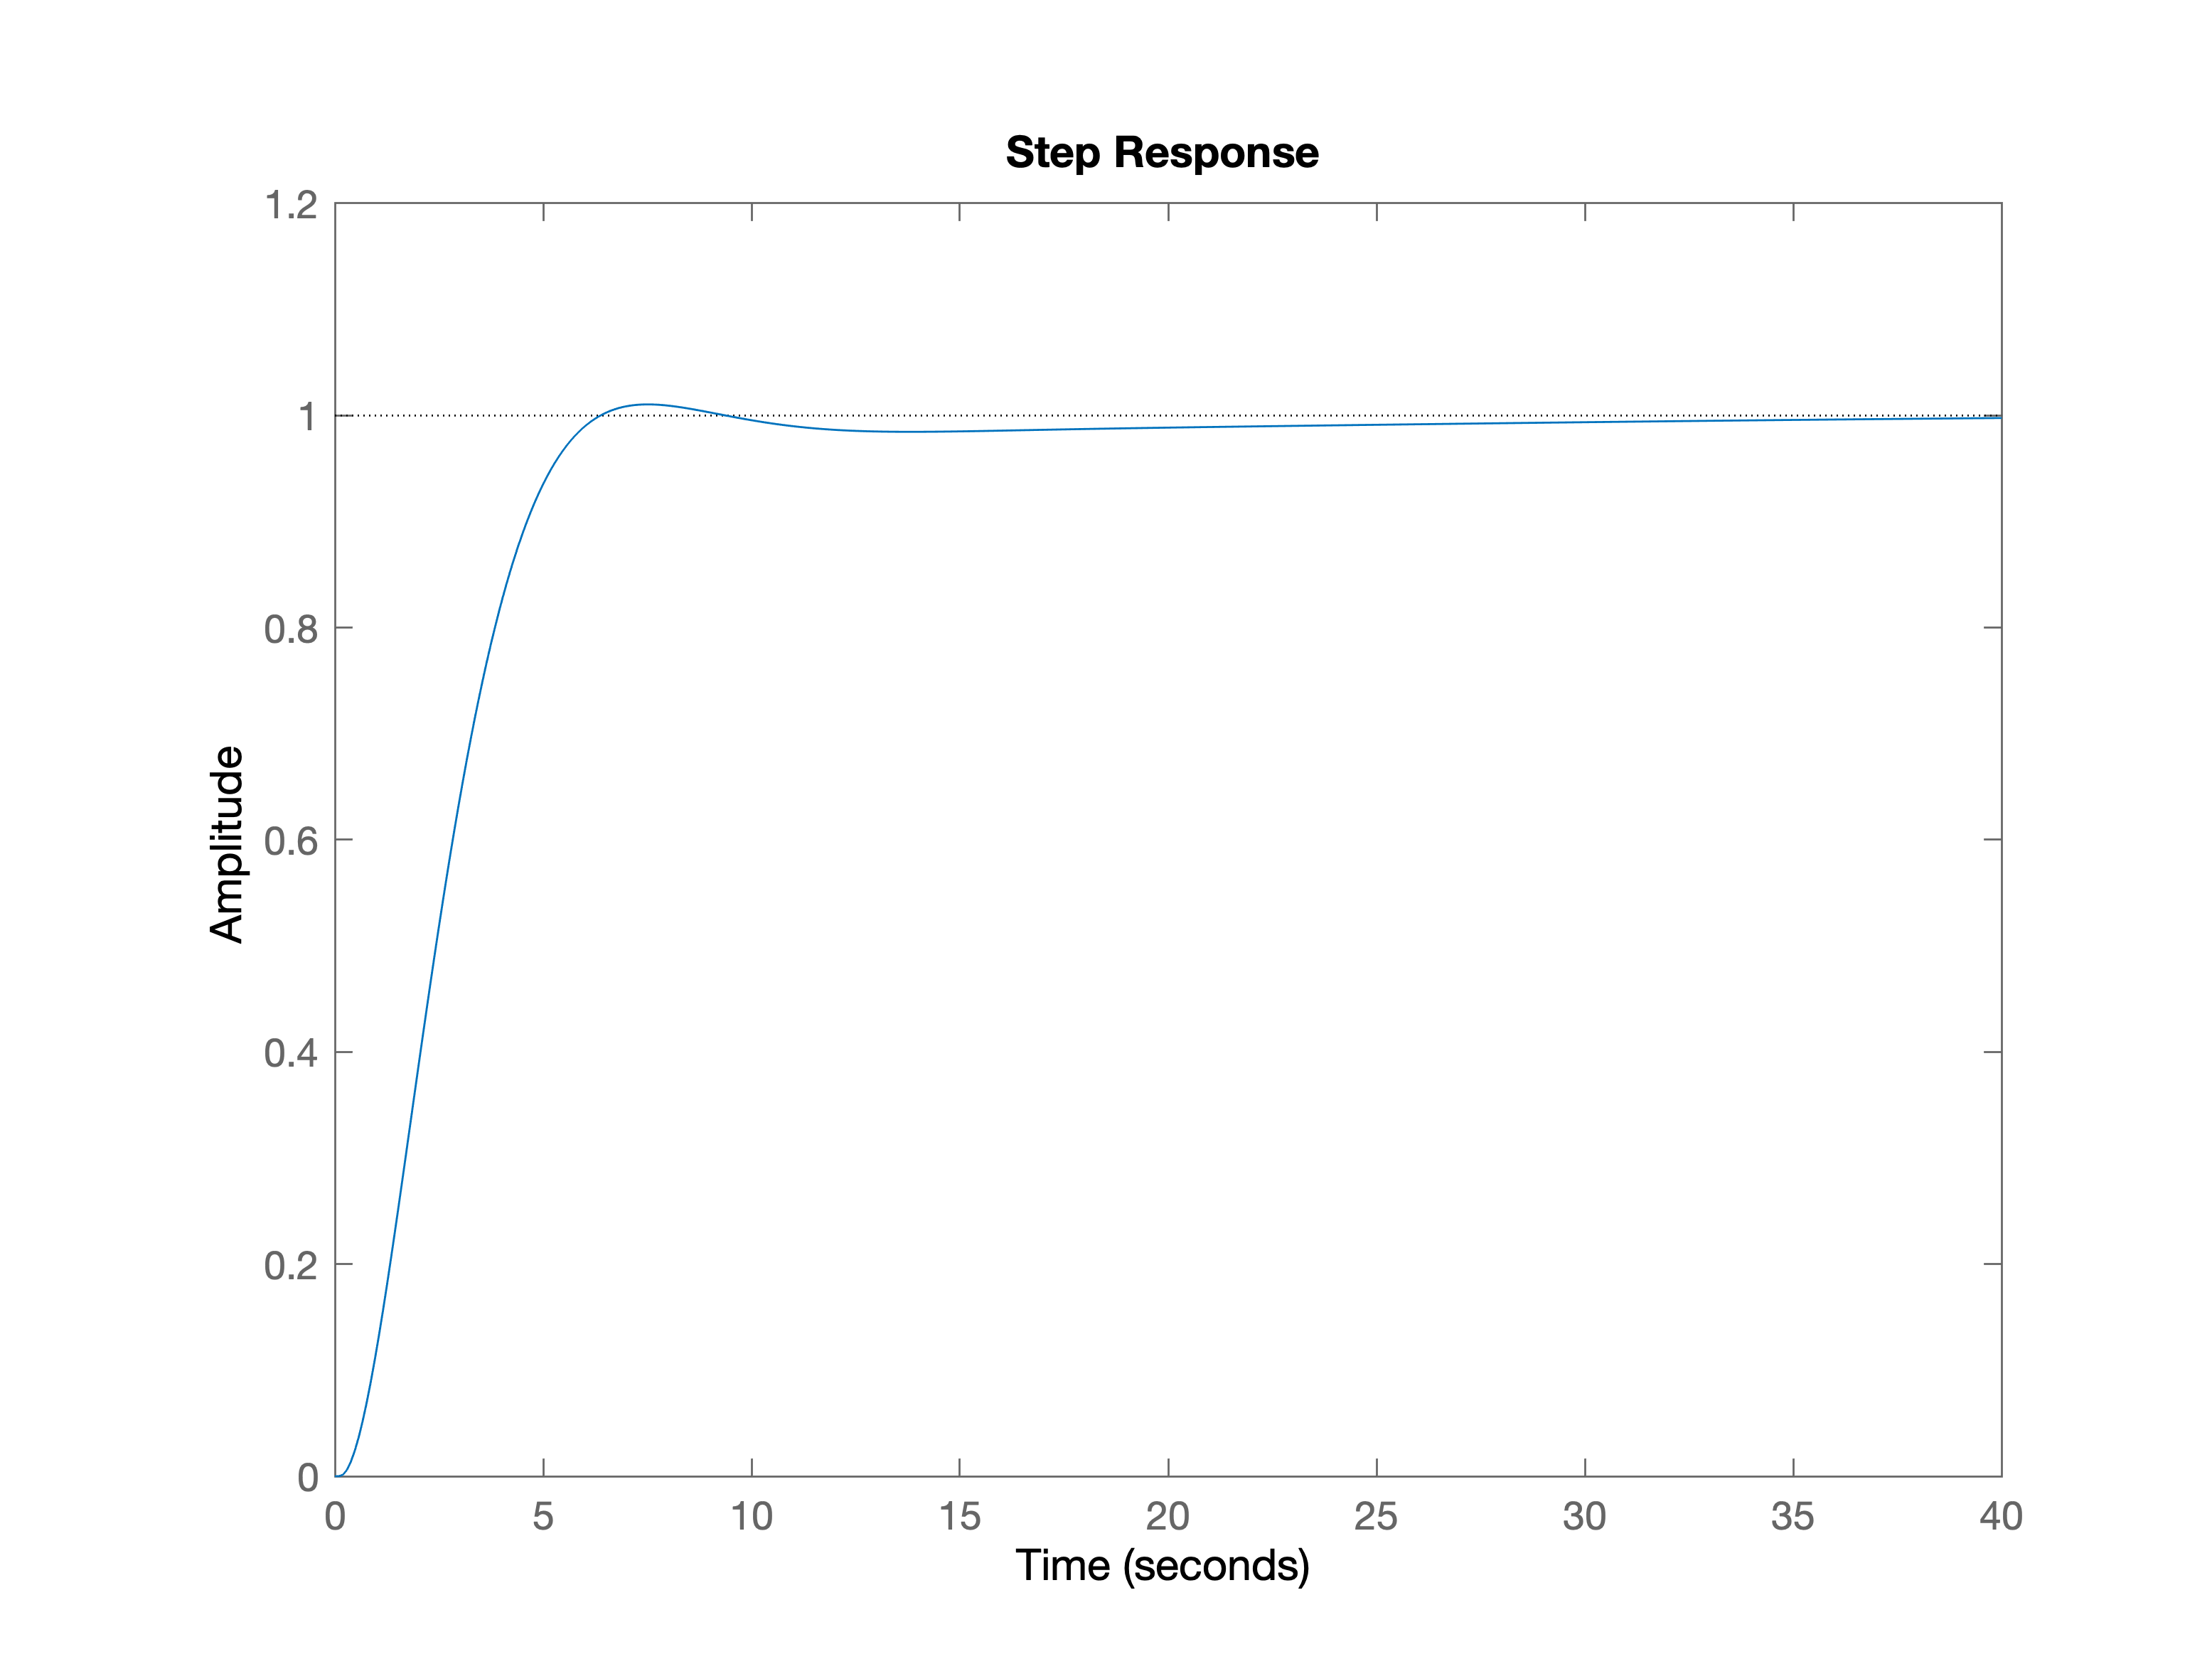
\includegraphics[width=12cm]{../Figure/P_I/PID.png}
	\centering
	\caption{خروجی پله واحد سیستم مدار بسته در حضور کنترل‌کننده PID}
	\label{PID}
\end{figure}
 بعد از طراحی در محیط SISO برای سیستم خطی، کنترل‌کننده طراحی در محیط غیرخطی نیز آورده شد و عملکرد قابل قبولی از خود نشان داد.
 خروجی پله نیم سیستم مدار بسته غیرخطی در حضور کنترل‌کننده PID در شکل
\ref{PID_non}
 آورده شده است.
   \begin{figure}[H]
 	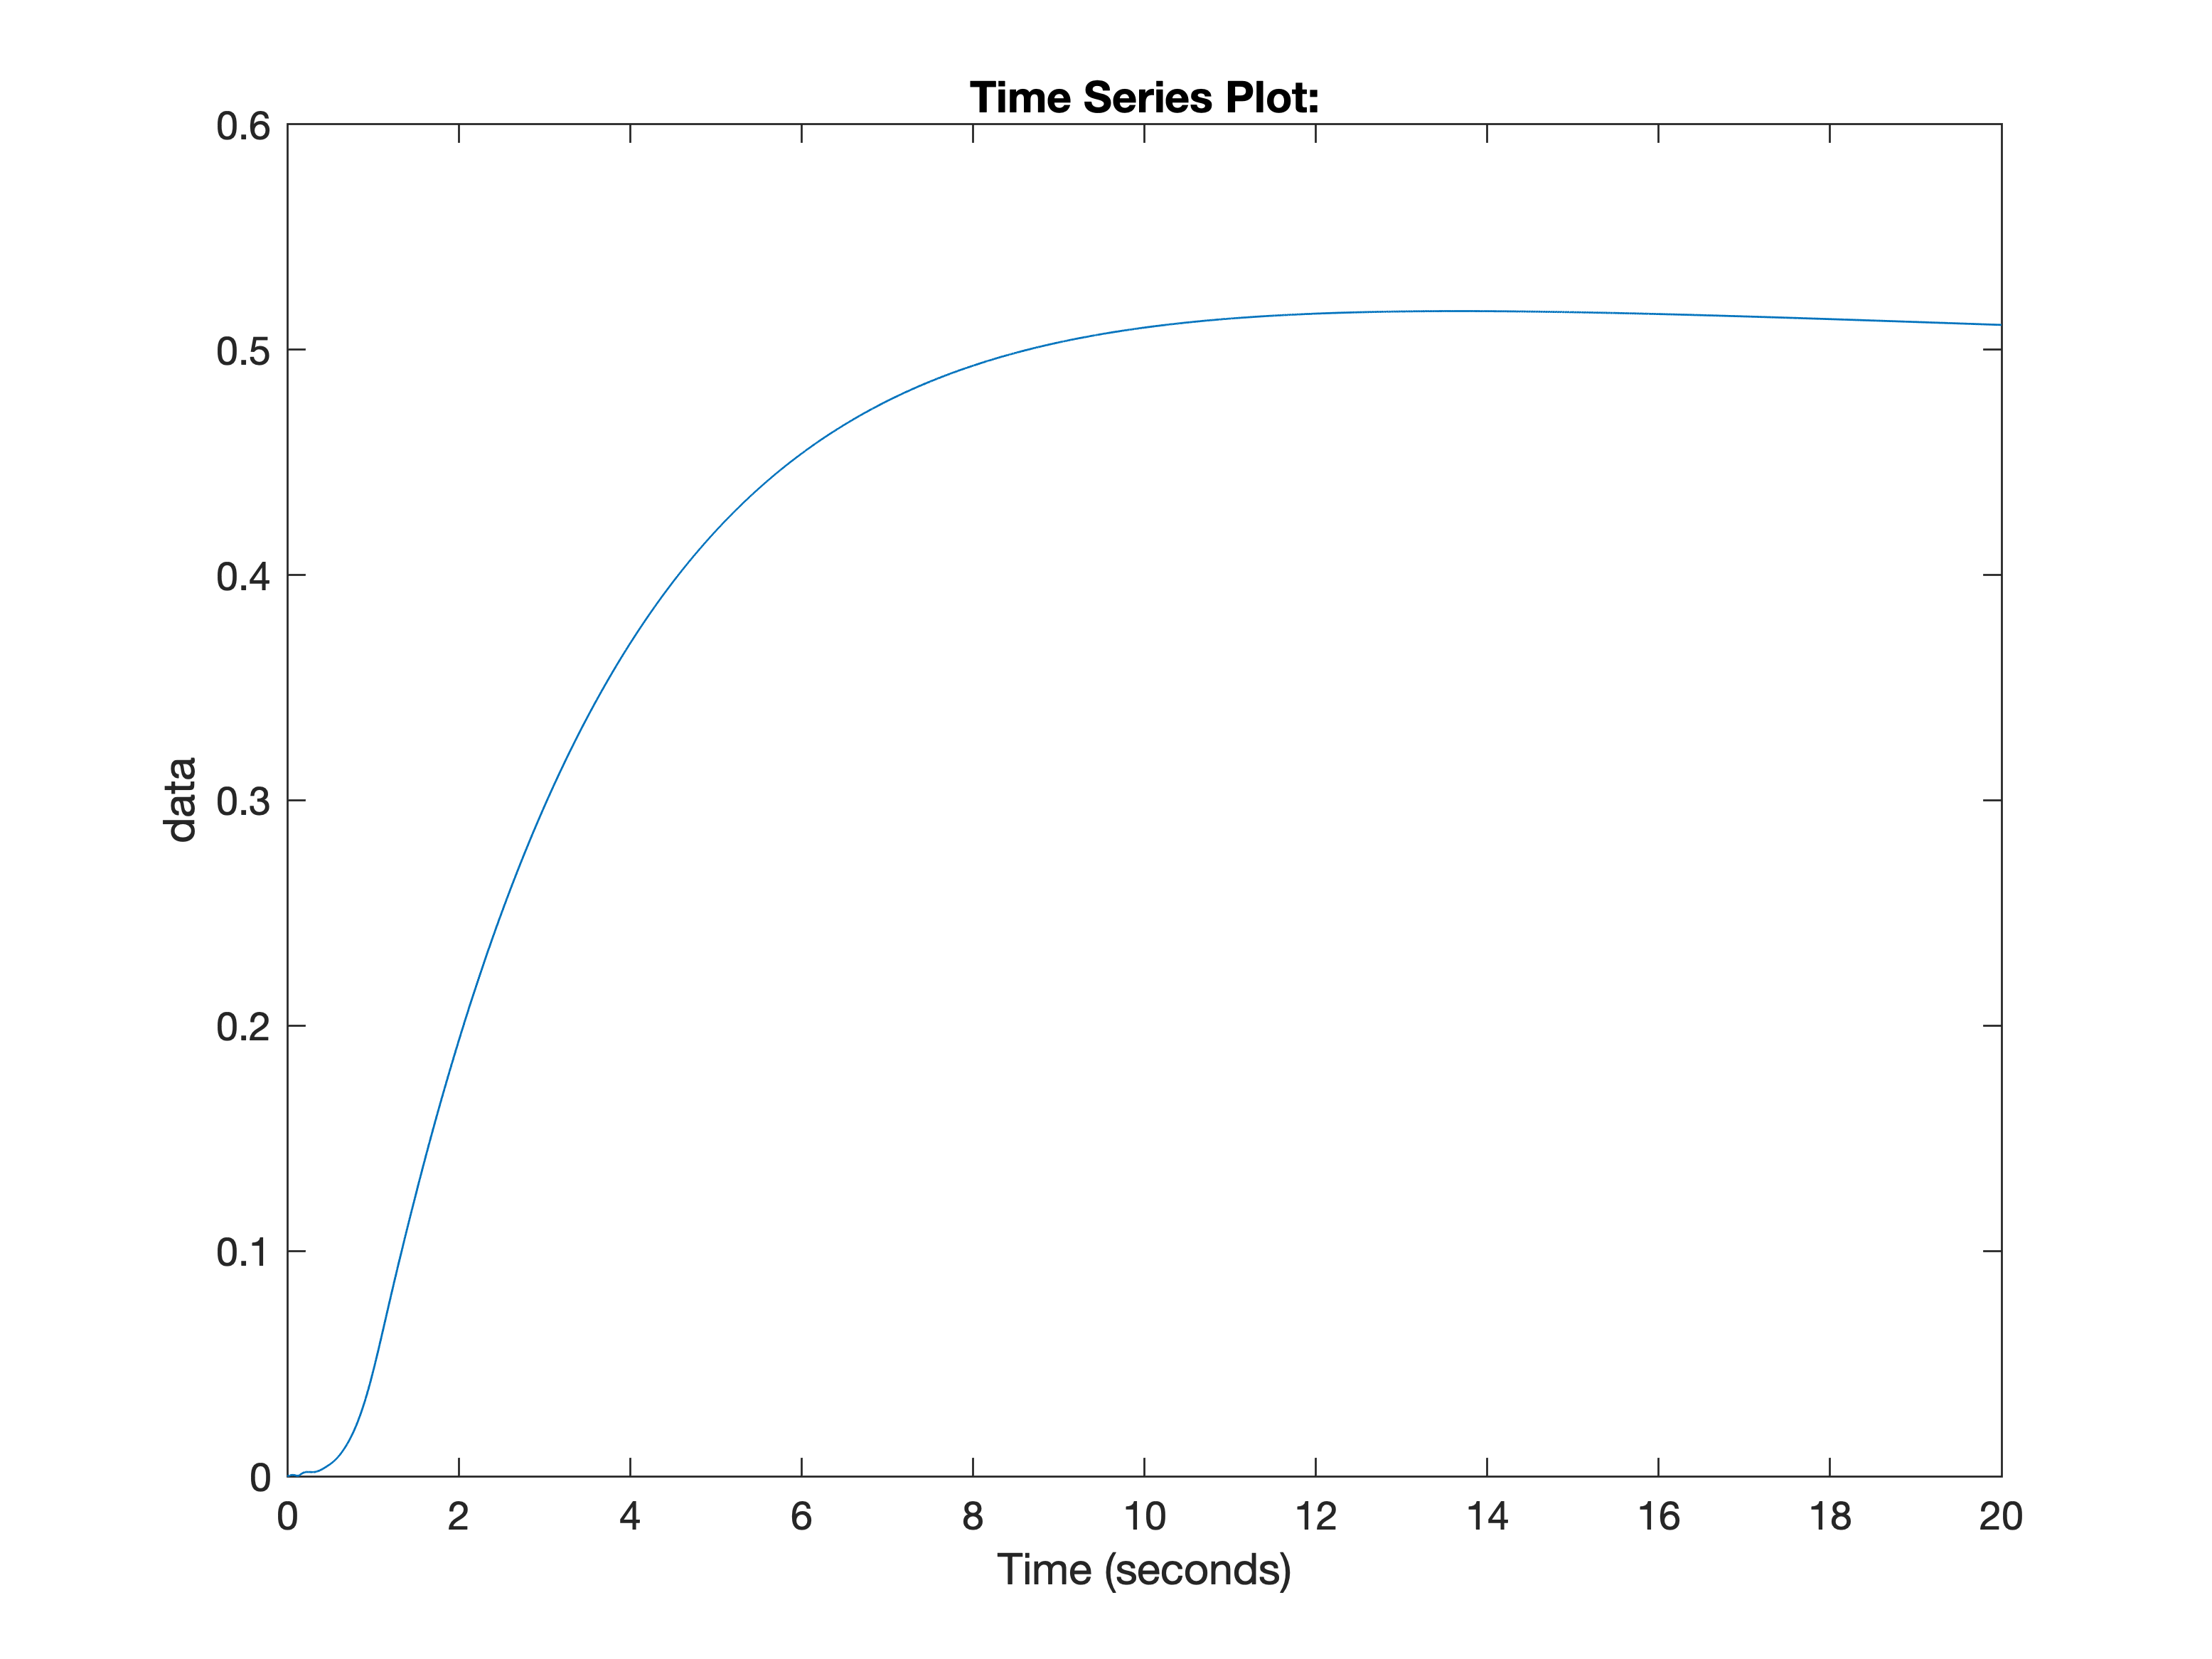
\includegraphics[width=12cm]{../Figure/P_I/PID_nonlinear.png}
 	\centering
 	\caption{خروجی پله واحد سیستم مدار بسته در حضور کنترل‌کننده PID}
 	\label{PID_non}
 \end{figure}
